\chapter{METODOLOGI}
\label{chap:metodologi}

Rancangan implementasi \emph{multi-tenancy} untuk \emph{provisioning}
klaster Kubernetes dimulai dari membuat aplikasi \emph{service} untuk \emph{provisioning}
yang terletak di komputer \emph{worker} untuk membuat
\emph{virtual machine}, kemudian membuat website \emph{dashboard} yang nantinya
digunakan oleh \emph{user} untuk membuat klaster Kubernetes secara dinamis dan sewaktu-waktu
menggunakan \emph{virtual machine} yang dibuat oleh aplikasi \emph{provisioning}.
Rancangan tahapan penyelesain implementasi tugas akhir ini
dapat dilihat pada gambar~\ref{fig:top-level-implementation}.

\begin{figure}[H]
  \centering
  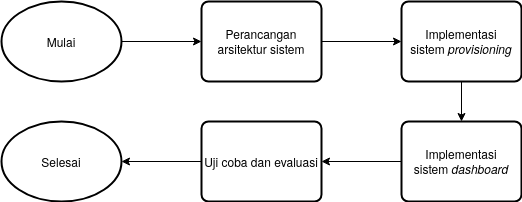
\includegraphics[scale=0.6]{gambar/top-level-implementation.png}
  \caption{Rancangan Penyelesaian Implementasi Tugas Akhir}
  \label{fig:top-level-implementation}
\end{figure}

Berdasarkan gambar \ref{fig:top-level-implementation} di atas, tahapan pertama
dalam rancangan implementasi tugas akhir adalah perancangan arsitektur sistem.
Tahapan perancangan arsitektur sistem berdasarkan kebutuhan sistem yang diperlukan
yaitu aplikasi \emph{website} sebagai \emph{dashboard} dan aplikasi \emph{provisioning}
untuk membuat \emph{virtual machine}. Setelah perancangan arsitektur sistem telah
selesai, implementasi dari rancangan sebelumnya akan dilakukan. Tahap terakhir
dari tugas akhir ini adalah uji coba dan evaluasi dari sistem yang telah dirancang.
Uji coba dan evaluasi ini bertujuan untuk memeriksa apakah sistem yang telah
diimplementasikan dapat berjalan sesuai kebutuhan dari tugas akhir ini.

\section{Perancangan Arsitektur Sistem}
\label{sec:perancanganarsitektursistem}

Secara garis besar, \emph{workflow} dari implementasi tugas akhir ini dapat dilihat
pada gambar \ref{fig:website-flowchart}. Selain itu, gambaran dari arsitektur sistem
implementasi tugas akhir ini terdapat
pada gambar \ref{fig:server-worker-top-level}. Berdasarkan gambar \ref{fig:server-worker-top-level},
komunikasi antara \emph{worker} dan server utama adalah komunikasi dua arah. Server utama
berkomunikasi dengan \emph{worker} untuk membuat \emph{virtual machine} dan \emph{worker}
berkomunikasi dengan server utama untuk memberi status bahwa \emph{worker} sudah siap
dalam menerima permintaan untuk membuat \emph{virtual machine} serta memberi status dari
pembuatan \emph{virtual machine}.

Setiap komputer fisik yang akan dijadikan \emph{worker} memerlukan aplikasi
atau sebuah \emph{service} yang dapat menerima permintaan pembuatan 
\emph{virtual machine} yang dikirimkan melalui server utama. Selain itu,
server utama juga memerlukan aplikasi yang dapat digunakan oleh pengguna
untuk membuat klaster dengan \emph{virtual machine} pada \emph{worker}.

\begin{figure}[H]
  \centering
  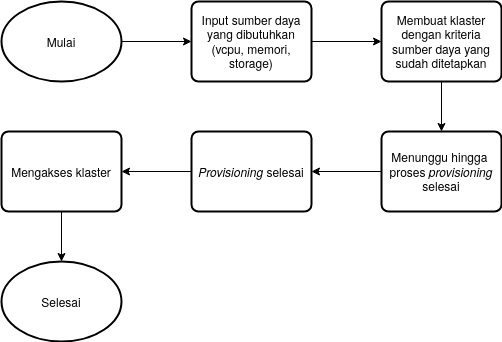
\includegraphics[scale=0.6]{gambar/flowchart-website.png}
  \caption{\emph{Workflow} Penggunaan Aplikasi}
  \label{fig:website-flowchart}
\end{figure}

\begin{figure}[H]
  \centering
  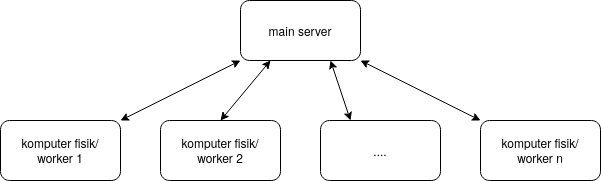
\includegraphics[scale=0.6]{gambar/server-worker-top-level.png}
  \caption{Gambaran Arsitektur Sistem}
  \label{fig:server-worker-top-level}
\end{figure}

\section{Implementasi Sistem \emph{Provisioning}}
\label{sec:implementasi-sistem-provisioning}

Sistem \emph{provisioning} pada setiap komputer \emph{worker} secara fungsi dapat dipisah
menjadi dua bagian besar, yaitu bagian server untuk menerimaa permintaan pembuatan klaster yang dikirim
oleh server utama dan bagian pembuatan \emph{virtual machine}.

\subsection{Server}
\label{sec:server}

Komputer \emph{worker} menerima \emph{request} pembuatan klaster melalui jaringan internet.
Oleh karena itu, \emph{worker} dapat menerima \emph{request} dengan membuka dan mendengarkan \emph{port}
untuk menerima \emph{request} dari server utama. Implementasi tugas akhir ini menggunakan protokol
RPC dengan gRPC untuk menerima \emph{request} tersebut.

\begin{lstlisting}[
  caption={Definisi Prosedur RPC pada Komputer \emph{Worker}},
  label={lst:rpc-procedure}
]
syntax = "proto3";

option go_package = "./services/model/proto-model";

enum Status {
  STATUS_UNSPECIFIED = 0;
  STATUS_AVAILABLE = 1;
  STATUS_UNAVAILABLE = 2;
}

message Empty {}

message CreateNodeRequirements {
  int64 cpu = 1;
  int64 memory = 2;
  int64 storage = 3;
}

// create master
message CreateMasterRequest {
  string token = 1;
  CreateNodeRequirements requirements = 2;
}

message CreateMasterResponse {
  string ip_address = 1;
}

// create worker
message CreateWorkerRequest {
  string token = 1;
  string ip_address = 2;
  CreateNodeRequirements requirements = 3;
}

message CreateWorkerResponse {}

service NodeService {
  rpc CreateMaster(CreateMasterRequest) returns (CreateMasterResponse) {}
  rpc CreateWorker(CreateWorkerRequest) returns (CreateWorkerResponse) {}
}
\end{lstlisting}

Kode sumber \ref{lst:rpc-procedure} menunjukkan fungsi atau prosedur
yang disediakan oleh \emph{worker} menggunakan protokol RPC. Untuk membuat prosedur
di gRPC, format yang dipakai adalah format Protobuf. Protobuf merupakan format
yang digunakan oleh gRPC sebagai \emph{Interface Definition Language}.

Prosedur yang sudah ditulis menggunakan Protobuf akan dikonversi
ke bahasa pemrograman yang diinginkan. Hasil konversi tersebut hanya
berupa fungsi atau prosedur tanpa isi. Isi atau \emph{logic} dari fungsi atau prosedur
tersebut harus dibuat sesuai dengan keinginan pengguna. Hasil konversi dari Protobuf
dapat dibagikan ke komputer lainnya yang memerlukan prosedur tersebut. 

Pada implementasi tugas akhir ini, komputer \emph{worker} menerima
hasil konversi dari prosedur dari Protobuf dan membuat isi dari
prosedur yang sudah ditetapkan. Server utama juga menerima hasil konversi
dan akan menggunakannya untuk menjalankan fungsi atau prosedur tersebut di komputer
\emph{worker}. Isi dari prosedur yang akan dijalankan di komputer \emph{worker} terdapat
pada kode sumber \ref{lst:isi-prosedur}. Isi prosedur tersebut adalah \emph{logic}
untuk membuat \emph{virtual machine} yang berjenis \emph{master node} atau \emph{worker node}.
Perbedaan dari keduanya adalah \emph{master node} akan bertugas menjadi \emph{control plane}
dari klaster Kubernetes yang dibuat nantinya.

\clearpage

\lstinputlisting[
  language=Go,
  caption={Isi Prosedur pada Komputer \emph{Worker}},
  label={lst:isi-prosedur}
]{program/rpc-procedure-logic.go}

\subsection{\emph{Provisioning}}
\label{sec:provisioning}

Setelah komputer menerima \emph{request} pembuatan klaster melalui RPC,
\emph{request} tersebut diteruskan ke sistem \emph{provisioning}.

\section{Implementasi Sistem \emph{Dashboard}}
\label{sec:implementas-sistem-dashboard}

\subsection{Uji Coba dan Evaluasi}
\label{sec:uji-coba-dan-evaluasi}

\section{Bahan dan Peralatan yang Digunakan}
\label{sec:implementasi alat}

Alat diimplementasikan dengan

% Contoh pembuatan potongan kode
% \begin{lstlisting}[
%   language=C++,
%   caption={Program halo dunia.},
%   label={lst:halodunia}
% ]
% #include <iostream>
%
% int main() {
%     std::cout << "Halo Dunia!";
%     return 0;
% }
% \end{lstlisting}
%
% % Contoh input potongan kode dari file
% \lstinputlisting[
%   language=Python,
%   caption={Program perhitungan bilangan prima.},
%   label={lst:bilanganprima}
% ]{program/bilangan-prima.py}
